\chapter{Empirical Evaluation}
\label{chap:evaluation}

We test several hypotheses in order to provide a thorough comparison of CPU versus GPU processing as well as online versus offline learning. This chapter contains detailed explanations of each experiment we ran, including why we ran the experiment, the environment setup, and a discussion of the results.

\section{Performance Scaling}

The performance of the GPU on tasks which benefit from parallel processing is not always better than the CPU. Remember that the GPU processes single threads slower than the CPU and is constrained by memory operations. As a result, the GPU shows its greatest performance gains as the size of the input scales. In fact, current generation GPUs hit peak performance for matrix operations when the matrix dimensions are close to $1024 \times 1024$ \cite{cuda:perf}. With that in mind we ran experiments to demonstrate the impact of this on LSPI as the size of the input scales.

There are two inputs for LSPI that scale, each of which we ran experiments to evaluate. The first experiment we ran tested the performance of LSPI as the number of samples to process increased. The experiment was setup by first collecting $150,000$ samples from an agent following a random policy with a $25\%$ exploration rate. We then separated these samples into groups of varying size ranging from $30,000$ to $150,000$. With each group of samples we trained an agent using the GPU implementation and then using the CPU implementation and measured the amount of time it took to converge on a policy. For consistency both implementations were executing the same code on the same hardware with the exception of the BLAS calls, which were unique to the specific implementation. The GPU implementation was executed inside of the Quake III engine by halting all operations until a policy was generated. Due to technical limitations, the CPU implementation would not function in the Quake III engine; however, we were able to execute the same code path outside of the Quake III engine to ensure the results would be consistent.

Figure \ref{fig:samples} shows the graph of our results complete with linear best-fit lines. We observe that the GPU implementation not only performs worse than the CPU implementation, but also appears to scale worse with the number of samples. At first glance, this may seem contrary to the expectations of our work. In reality, these results are both reasonable and expected. In order to minimize the performance impact of the basis function we chose to run these tests with the smallest basis function, which had $30$ values. The result is that the largest matrix computation involves $30 \times 30$ or $90$ operations. A CPU is capable of processing this number of operations in a very short period of time, and does not have to do any memory copy operations before processing the samples. The GPU can compute most of these operations in parallel; however, first all of the samples must be copied from host memory to device memory. The end result is that with such a small basis the CPU performs better and because the GPU must always do a memory copy, the CPU also scales better.

\begin{figure}
	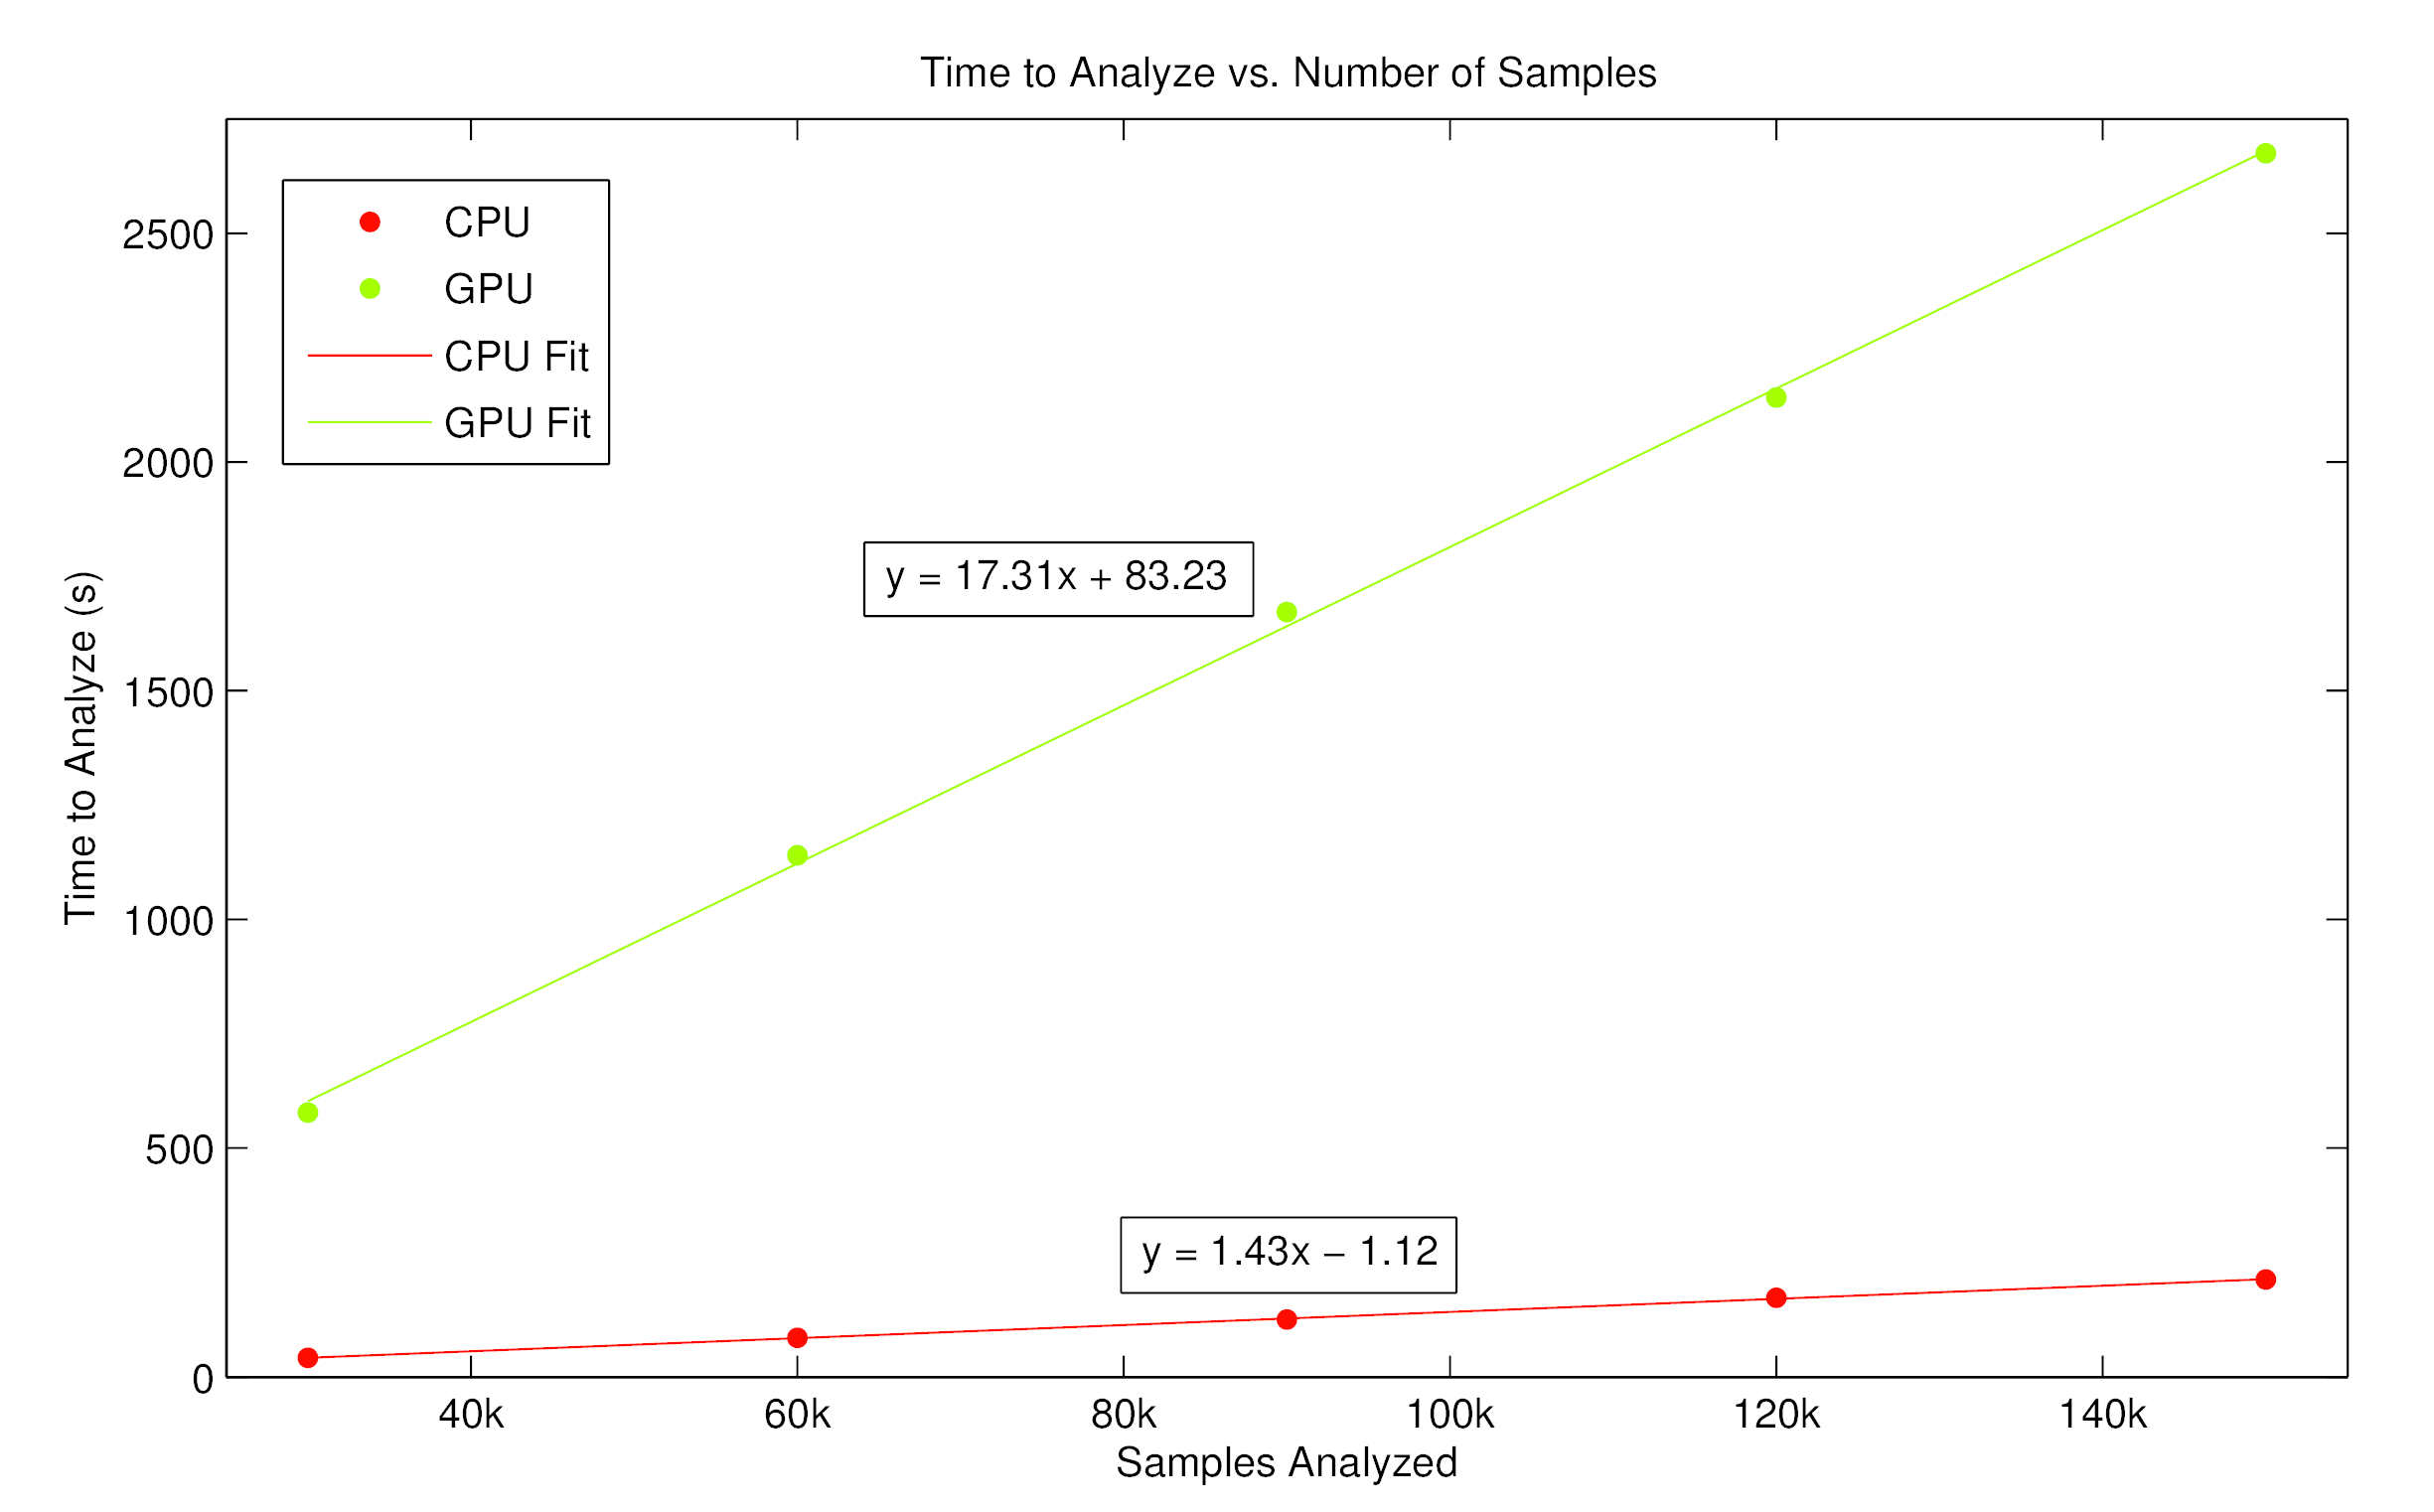
\includegraphics[width=\textwidth]{Time_vs_Samples.png}
    \caption{Plot of performance based on sample size}
	\label{fig:samples}
\end{figure}

The second experiment tested the performance of LSPI with a constant number of samples while the basis size increased. The experiment was setup by collecting $10,000$ samples from an agent following a random policy with a $25\%$ exploration rate. These samples were then used to train agents with basis functions which ranged in size from $30$ to $258$. As with the samples scaling experiment, every attempt was made to ensure these experiments were completed in identical environments. Due to the variance we witnessed in our experiments we repeated this training for each agent three times for both the CPU and GPU implementation. The results are graphed with fit lines in Figure \ref{fig:basis}.

\begin{figure}
    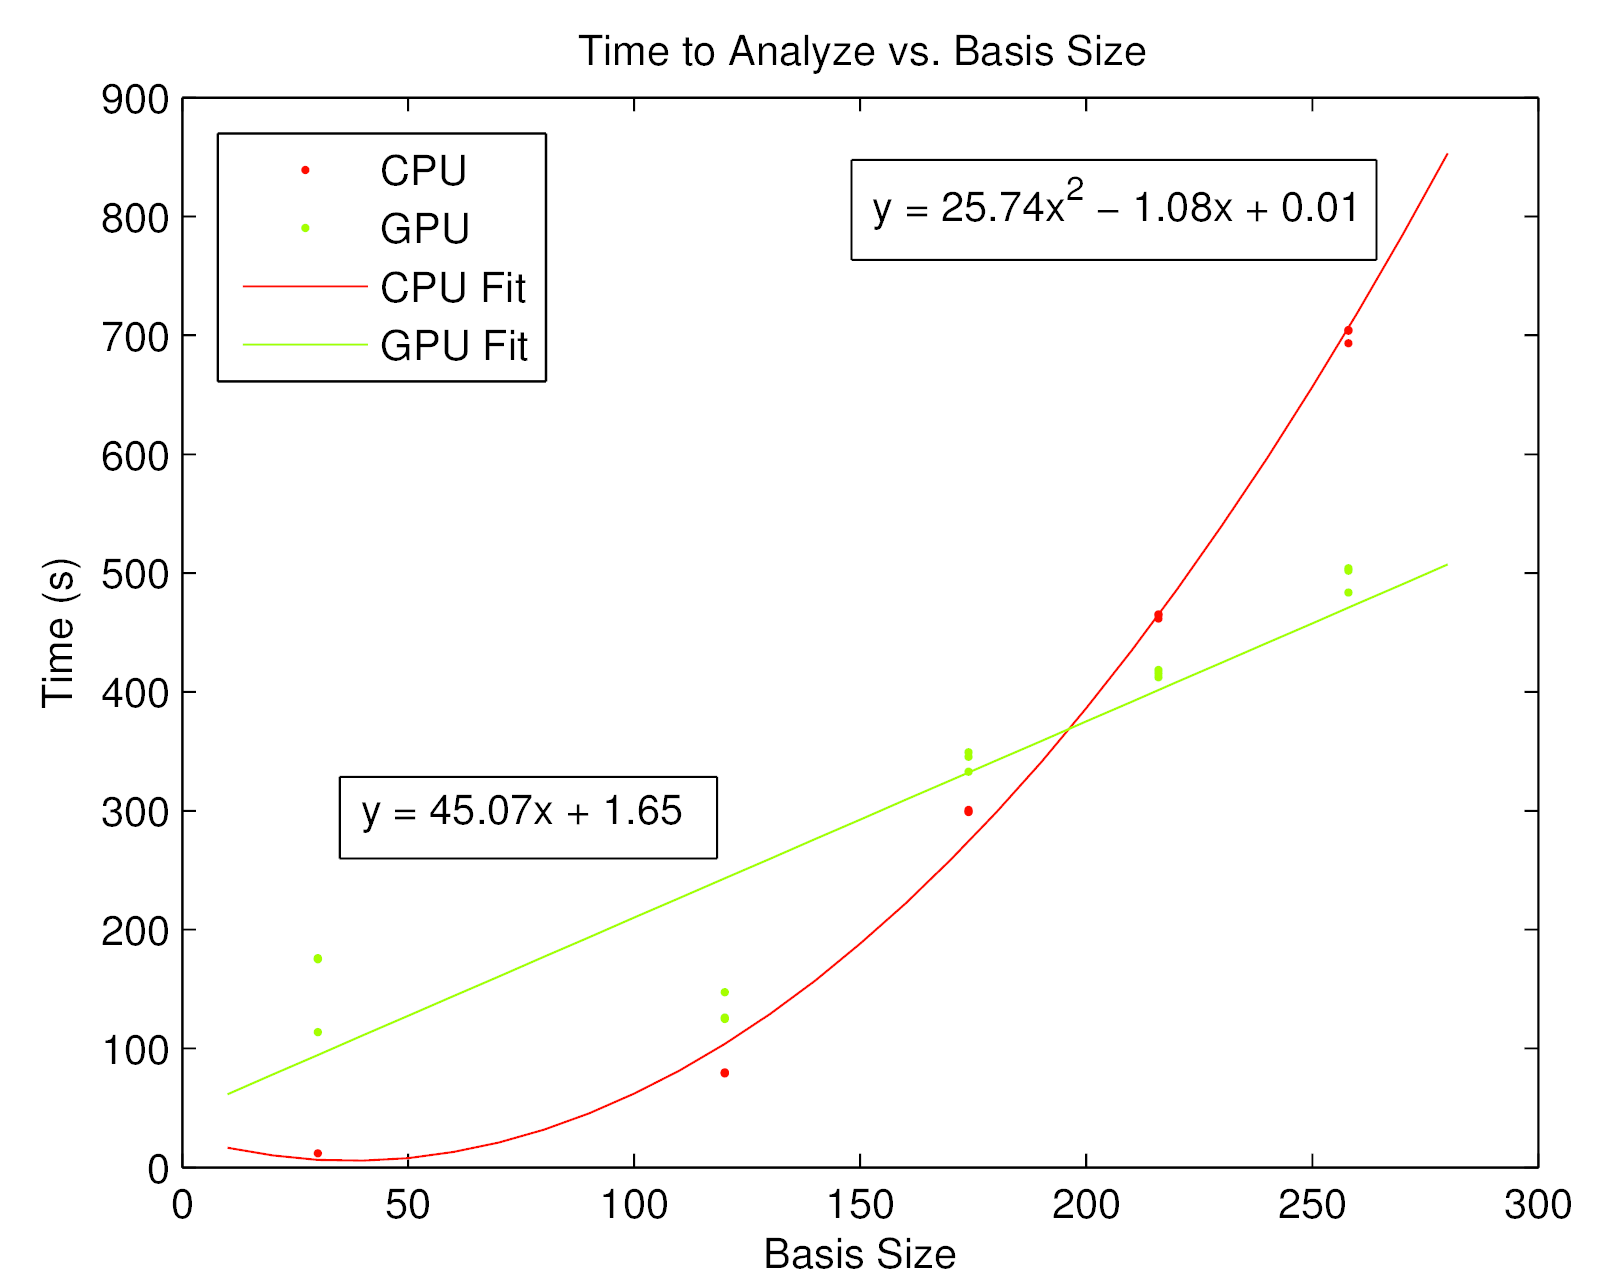
\includegraphics[width=\textwidth]{Time_vs_Basis.png}
    \caption{Plot of performance based on basis size}
    \label{fig:basis}
\end{figure}

Based on the data we collected, it is clear that while the GPU performs slower than the CPU with small basis sizes, the GPU scales well with increasing basis size. For our particular configuration the performance crossover occurs around $200$; however, that intersection point will vary based on the specific hardware configurations as well as the optimizations used to improve performance.

While the speeds we measured on the CPU were relatively stable, we noticed a high level of variance in our measurements for the GPU. Based on our knowledge of how linear algebra operations scale on the GPU, we would expect LSPI to scale approximately linearly on the GPU. Most of our data supports this; however, there are some outliers present on the graph.

When we measured the time to analyze the samples using a basis size of $120$ we were consistently seeing results that were comparable to the amount of time needed to analyze the samples using a basis of size $30$. To understand this result, we must first understand what factors will impact the amount of time needed to execute LSPI.

At its core, LSPI can be viewed as an optimization algorithm which iteratively executes the algorithm LSTD$Q$ in an attempt to locate the policy which maximizes the utility of the agent for the given samples. Depending on both the samples and the basis function used to evaluate the samples, the number of iterations of LSTD$Q$ necessary can change. Looking at Figure \ref{fig:basis} the data shows that although it is less noticeable, all three tests for the CPU also appear under the curve. This suggests that the particular features we selected may have had an impact on the number of iterations of LSTD$Q$ required to converge.

Another potential contributing factor to this result is the nature of the GPU architecture. When code is executed on the GPU, some number of processing units is allocated. The number of processing units allocated does not necessarily correspond with the size of the data input. As a result, there may be processing units which are effectively idle. The end result is that two operations with different input sizes may take the same amount of time. Between the architecture of the GPU and the interaction of the basis features with the speed of convergence, we feel that these results still fall within the expected range.

When it came time to plot fit lines for the data, the choice was obvious for the CPU: the results very clearly represent a second degree polynomial, with $R^2 = 0.99$. For the GPU the choice was less obvious, particularly since the outlier at $120$ made any fit difficult. We chose a linear fit because the data fits a linear model better with the outliers removed. The fit was less consistent for the GPU data with $R^2 = 0.7987$.

It is important to keep in mind that the point at which the GPU overtakes the CPU in performance will vary based on specific hardware configurations, as well as the level of optimization put into the implementation. As stated earlier, we chose to optimize very little to focus on the scaling performance gains. Furthermore, unless the CPU implementation was capable of being optimized at a rate much higher than the GPU optimizations, these performance tweaks would only serve to lower the barrier for seeing improvements with the GPU.

In our experiments we were able to generate very good policies with a very small basis function; however, this is largely due to the amount of hand written scripts our bot relies on to interact with the environment. While this allowed us to test the performance of LSPI under different conditions very well, our AI implementation does not do allow more complex behavior to be learned, limiting the benefits observed using reinforcement learning.

To understand the benefits of a large basis function, consider designing an AI agent for Quake III from the ground up. In order to manage the complexity of the environment, it is helpful to have some basic actions available to the agent: \emph{attack}, \emph{get health}, \emph{get weapon}, \emph{get armor}, \emph{get powerup}, \emph{search for enemy}, \emph{defend location}, \emph{flee from enemy}, \emph{change weapon}, \emph{reload}. Already our agent has more actions available than the implementation was used for testing.

Now that we have defined some actions for our agent, consider what information would be useful in order to make intelligent decisions. First and foremost, the agent needs information on its own state: \emph{health}, \emph{armor}, \emph{equipped weapon}, \emph{available weapons}, \emph{equipped ammo}, \emph{available ammo}. Keep in mind that some of these features, such as equipped weapon and available weapons, would need to be represented by multiple values in the basis. In fact, representing this information in Quake III would already result in a basis with $23$ values which must be repeated for each of the $10$ actions we have defined for a total size of $230$, and we still lack the information to make more complex decisions such as how to choose an area to defend.

The basis size can be made smaller by carefully controlling the basic actions available to the bot and carefully selecting features; however, the key result of this experiment is demonstrating that the advent of GPU acceleration enables an AI designer more control over selecting features and actions for an agent without suffering the significant performance degradation present with CPU based algorithms as the basis size increases.

\section{Online LSPI}

\subsection{Policy Gradient}

The term \emph{Policy Gradient} describes a class of machine learning techniques which apply gradient ascent optimization to determine the optimal policy. Given the policy value function, $p(\theta)$, policy gradient algorithms can be succinctly described by the following formula:

\[
    \theta_{n+1} = \theta_{n} + \alpha\nabla_\theta p(\theta_{n})
\]
where $\theta$ represents the policy parameters and $\alpha$ is referred to as the step size or learning rate \cite{norvig}\cite{bishop}.

Before we estimate $\nabla_\theta p(\theta)$, we must ensure that $p(\theta)$ is differentiable with respect to $\theta$. Assume we have a basis function, $J_\theta(s,a)$ which is used to generate a policy as follows:

\[
    \pi_\theta(s,a) = \argmax_a J_\theta(s,a)
\]
The use of the $argmax$ function may result in a discontinuous distribution. This can be fixed by using a probabilistic policy \cite{olpomdp:lecture}:

\begin{equation}
\label{eq:grad:policy}
    \pi_\theta(s,a) = Pr(a|s) = \frac{e^{J_\theta(s,a)/T}}{\sum\limits_{a'\in A} e^{J_\theta(s,a')/T}}
\end{equation}

To estimate the gradient from samples we use the following formula:
\begin{equation}
\label{eq:grad}
    \begin{aligned}
        \nabla_\theta p(\theta) &= \sum_a\pi_\theta(s_0,a)g_\theta(s_0,a)R(a) \\
        g_\theta(s_0,a) &= f_\theta(s_0, a) - \sum\limits_{a'} \pi_\theta(s_0,a')f_\theta(s_0,a')
    \end{aligned}
\end{equation}

Equation \ref{eq:grad} is the basis for an online algorithm called OLPOMDP \cite{olpomdp}. Intuitively, the algorithm estimates the gradient using Monte Carlo techniques: execute the policy while making small changes to $\theta$. Because we use Equation \ref{eq:grad:policy} to select actions, our agent will naturally explore the environment. With each action we then update the value $e$, called the eligibility trace, by estimating the value of the gradient for that action.

The pseudocode for OLPOMDP is given in Algorithm \ref{olpomdp}. Notice that instead of updating $\theta$ directly the value $e$, called the eligibility trace, is used as an intermediary. The eligibility trace represents the discounted sum of gradients over previous state-action pairs and is used to update $\theta$ according to the reward given for the corresponding action. The value $\beta$ is referred to as the bias and controls the weight of previous experiences in the environment. Increasing $\beta$ biases the algorithm toward past experiences while also increasing the variance. 

\begin{algorithm}
\caption{OLPOMDP}
\label{olpomdp}
    {\fontsize{12}{10}\selectfont
    \begin{algorithmic}[1]
        \REQUIRE
            \begin{itemize} 
                \item $\beta \in [0,1)$ 
                \item $T > 0$ 
                \item $\theta_0 \in \mathbb{R}^K$ 
            \end{itemize}
    \STATE Set $e = 0$
    \FOR{$t = 0$ to $\infty$}
        \STATE Observe the current state, $s$
        \STATE Select action $a$ according to $\pi_\theta(s)$
        \STATE Execute $a$
        \STATE Observe reward $r$
        \STATE $e \leftarrow \beta e + f(s,a) - \sum\limits_{a'}\pi_\theta(s,a')f_\theta(s,a')$
        \STATE $\theta \leftarrow + \alpha \cdot r \cdot e$
    \ENDFOR
    \end{algorithmic}
    }
\end{algorithm}

\section{Bot Reward}